\documentclass[12pt, titlepage]{article}

\usepackage{fullpage}
\usepackage[round]{natbib}
\usepackage{multirow}
\usepackage{booktabs}
\usepackage{tabularx}
\usepackage{graphicx}
\usepackage{float}
\usepackage{hyperref}
\hypersetup{
    colorlinks,
    citecolor=black,
    filecolor=black,
    linkcolor=red,
    urlcolor=blue
}
\usepackage[round]{natbib}

\newcounter{acnum}
\newcommand{\actheacnum}{AC\theacnum}
\newcommand{\acref}[1]{AC\ref{#1}}

\newcounter{ucnum}
\newcommand{\uctheucnum}{UC\theucnum}
\newcommand{\uref}[1]{UC\ref{#1}}

\newcounter{mnum}
\newcommand{\mthemnum}{M\themnum}
\newcommand{\mref}[1]{M\ref{#1}}

\title{SE 3XA3: Module Guide\\Jumble Words}

\author{Team 08, Shunbill Jumble
	\\Shesan Balachandran, balacs1
	\\Bill Nguyen, nguyew3
	\\Muneeb Arshad, arsham14
}


\date{\today}

% \input{../../Comments}

\begin{document}

\maketitle

\clearpage
\begin{table}[bp]
	\caption{\bf Revision History}
	\begin{tabularx}{\textwidth}{p{3cm}p{2cm}X}
		\toprule {\bf Date} & {\bf Version} & {\bf Notes}\\
		\midrule
		March 15 2021 & 0.0 & Initial Draft\\
		\bottomrule
	\end{tabularx}
\end{table}
\clearpage
\pagenumbering{roman}
\tableofcontents
\listoftables
\listoffigures



\newpage

\pagenumbering{arabic}

\section{Introduction}

Decomposing a system into modules is a commonly accepted approach to developing
software.  A module is a work assignment for a programmer or programming
team~\citep{ParnasEtAl1984}.  We advocate a decomposition
based on the principle of information hiding~\citep{Parnas1972a}.  This
principle supports design for change, because the ``secrets'' that each module
hides represent likely future changes.  Design for change is valuable in SC,
where modifications are frequent, especially during initial development as the
solution space is explored.  

Our design follows the rules layed out by \citet{ParnasEtAl1984}, as follows:
\begin{itemize}
\item System details that are likely to change independently should be the
  secrets of separate modules.
\item Each data structure is used in only one module.
\item Any other program that requires information stored in a module's data
  structures must obtain it by calling access programs belonging to that module.
\end{itemize}

After completing the first stage of the design, the Software Requirements
Specification (SRS), the Module Guide (MG) is developed~\citep{ParnasEtAl1984}. The MG
specifies the modular structure of the system and is intended to allow both
designers and maintainers to easily identify the parts of the software.  The
potential readers of this document are as follows:

\begin{itemize}
\item New project members: This document can be a guide for a new project member
  to easily understand the overall structure and quickly find the
  relevant modules they are searching for.
\item Maintainers: The hierarchical structure of the module guide improves the
  maintainers' understanding when they need to make changes to the system. It is
  important for a maintainer to update the relevant sections of the document
  after changes have been made.
\item Designers: Once the module guide has been written, it can be used to
  check for consistency, feasibility and flexibility. Designers can verify the
  system in various ways, such as consistency among modules, feasibility of the
  decomposition, and flexibility of the design.
\end{itemize}

The rest of the document is organized as follows. Section
\ref{SecChange} lists the anticipated and unlikely changes of the software
requirements. Section \ref{SecMH} summarizes the module decomposition that
was constructed according to the likely changes. Section \ref{SecConnection}
specifies the connections between the software requirements and the
modules. Section \ref{SecMD} gives a detailed description of the
modules. Section \ref{SecTM} includes two traceability matrices. One checks
the completeness of the design against the requirements provided in the SRS. The
other shows the relation between anticipated changes and the modules. Section
\ref{SecUse} describes the use relation between modules.

\section{Anticipated and Unlikely Changes} \label{SecChange}

This section lists possible changes to the system. According to the likeliness
of the change, the possible changes are classified into two
categories. Anticipated changes are listed in Section \ref{SecAchange}, and
unlikely changes are listed in Section \ref{SecUchange}.

\subsection{Anticipated Changes} \label{SecAchange}

Anticipated changes are the source of the information that is to be hidden
inside the modules. Ideally, changing one of the anticipated changes will only
require changing the one module that hides the associated decision. The approach
adapted here is called design for
change.

\begin{description}
\item[\refstepcounter{acnum} \actheacnum \label{acHardware}:] The specific
  hardware on which the software is running.
\item[\refstepcounter{acnum} \actheacnum \label{acInput}:] The format of the
  initial input data.
\item[\refstepcounter{acnum} \actheacnum \label{acInput}:] The format of the leaderboard display (adding more scores in the leaderboard, change the way the leaderboard is ordered)
\item[\refstepcounter{acnum} \actheacnum \label{acInput}:] adding more categories for the user to choose from
\item[\refstepcounter{acnum} \actheacnum \label{acInput}:] The format of difficulty level (currently have difficulty based on length of words can be also lower the amount of time based on difficulty setting)
\item[\refstepcounter{acnum} \actheacnum \label{acInput}:] The GUIs for the display of the game, main menu and settings
\item[\refstepcounter{acnum} \actheacnum \label{acInput}:] Currently using external files for data such as words and leaderboard, can change all data storage to an actual database such as postgres
\end{description}

\subsection{Unlikely Changes} \label{SecUchange}

The module design should be as general as possible. However, a general system is
more complex. Sometimes this complexity is not necessary. Fixing some design
decisions at the system architecture stage can simplify the software design. If
these decision should later need to be changed, then many parts of the design
will potentially need to be modified. Hence, it is not intended that these
decisions will be changed.

\begin{description}
\item[\refstepcounter{ucnum} \uctheucnum \label{ucIO}:] Input/Output devices
  (Input: File and/or Keyboard, Output: File, Memory, and/or Screen).
\item[\refstepcounter{ucnum} \uctheucnum \label{ucInput}:] There will always be
  a source of input data external to the software.
\item[\refstepcounter{ucnum} \uctheucnum \label{ucInput}:] There will be an external output file for the leader board so external storage required.
\item[\refstepcounter{ucnum} \uctheucnum \label{ucInput}:] The game logic for calculating points for leader boards.
\end{description}

\section{Module Hierarchy} \label{SecMH}

This section provides an overview of the module design. Modules are summarized
in a hierarchy decomposed by secrets in Table \ref{TblMH}. The modules listed
below, which are leaves in the hierarchy tree, are the modules that will
actually be implemented.

\begin{description}
\item [\refstepcounter{mnum} \mthemnum \label{mHH}:] Main GUI Module
\item [\refstepcounter{mnum} \mthemnum \label{mHH}:] Settings Module
\item [\refstepcounter{mnum} \mthemnum \label{mHH}:] Settings GUI Module
\item [\refstepcounter{mnum} \mthemnum \label{mHH}:] Game Control Module
\item [\refstepcounter{mnum} \mthemnum \label{mHH}:] User GUI Module
\item [\refstepcounter{mnum} \mthemnum \label{mHH}:] User Module
\item [\refstepcounter{mnum} \mthemnum \label{mHH}:] Leaderboard Module
\end{description}


\begin{table}[h!]
\centering
\begin{tabular}{p{0.3\textwidth} p{0.6\textwidth}}
\toprule
\textbf{Level 1} & \textbf{Level 2}\\
\midrule

{Hardware-Hiding Module} & ~ \\
\midrule

\multirow{7}{0.3\textwidth}{Behaviour-Hiding Module}
& Main GUI Module\\
& Settings Module\\
& Settings GUI Module\\
& Game Control Module\\
& User GUI Module\\
\midrule

\multirow{3}{0.3\textwidth}{Software Decision Module}
& User Module\\
& Leaderboard Module\\
\bottomrule

\end{tabular}
\caption{Module Hierarchy}
\label{TblMH}
\end{table}

\section{Connection Between Requirements and Design} \label{SecConnection}

The design of the system is intended to satisfy the requirements developed in
the SRS. In this stage, the system is decomposed into modules. The connection
between requirements and modules is listed in Table \ref{TblRT}.

The requirements described from the SRS can be described in a way that will allow the user to start/initiate the program, play the game correctly, while also being able to view aspects such as the leaderboard, and also modify the necessary settings such as game mode, difficulty level and categories. The modules that were mentioned in section 3 are going to be implemented in order to get full functionality for the program. To start the MainGUI Module helps to make certain that user can access the program/game and that the display/functionality of the main menu works as intended. The Settings Module helps make certain that the user is able to configure settings and that the settings (game mode, difficulty level and category) that are configured by the user are set correctly. The GameControl Module helps ensure that the game functionality is working as intended such when guessing a correct word the score updates, when the user wants to return to main menu the user will return to the main menu etc. The User GUI Module helps make certain that the display of the username menu is displayed properly and everything is initialized as intended. The User Module ensures the functionality of the user is working as intended such as when a new user is added it gets added properly, when a new score is recorded it updates the score of the user properly etc. Finally the Leaderboard Module helps make certain that the program will display the correct top ten usernames and scores from highest to lowest and that it gets updated accordingly.

\section{Module Decomposition} \label{SecMD}

Modules are decomposed according to the principle of ``information hiding''
proposed by \citet{ParnasEtAl1984}. The \emph{Secrets} field in a module
decomposition is a brief statement of the design decision hidden by the
module. The \emph{Services} field specifies \emph{what} the module will do
without documenting \emph{how} to do it. For each module, a suggestion for the
implementing software is given under the \emph{Implemented By} title. If the
entry is \emph{OS}, this means that the module is provided by the operating
system or by standard programming language libraries.  Also indicate if the
module will be implemented specifically for the software.

Only the leaf modules in the
hierarchy have to be implemented. If a dash (\emph{--}) is shown, this means
that the module is not a leaf and will not have to be implemented. Whether or
not this module is implemented depends on the programming language
selected.

\subsection{Hardware Hiding Modules}

\subsection{Behaviour-Hiding Module}

\subsubsection{Main GUI Module (M1)}

\begin{description}
\item[Secrets:]Functionalities of the main screen.
\item[Services:]Start game, leaderboard and quit game functionalities
\item[Implemented By:] [TkInter, Python3]
\end{description}

\subsubsection{Settings Module (M2)}

\begin{description}
\item[Secrets:]Manipulate game settings.
\item[Services:]Change difficulty, game mode, categories. 
\item[Implemented By:] [Python3]
\end{description}

\subsubsection{Settings GUI Module (M3)}

\begin{description}
\item[Secrets:]User interface elements including buttons and labels
\item[Services:]Select game difficulty, game mode, and categories through buttons
\item[Implemented By:] [TkInter, Python3]
\end{description}

\subsubsection{Game Control Module (M4)}

\begin{description}
\item[Secrets:]Manipulate game related interactions.
\item[Services:]Submit answer, guess word, go to next question or go back to main menu. 
\item[Implemented By:] [Python3]
\end{description}

\subsubsection{User GUI Module (M5)}

\begin{description}
\item[Secrets:]Display user related elements.
\item[Services:]Input username and submit username
\item[Implemented By:] [TkInter, Python3]
\end{description}

\subsection{Software Decision Module}

\subsubsection{User Module (M6)}

\begin{description}
\item[Secrets:]Manages the user information.
\item[Services:]Provide functionalities to insert, delete and update user data
\item[Implemented By:] [Python3]
\end{description}

\subsubsection{Leader board Module (M7)}

\begin{description}
\item[Secrets:]Manage the user high-scores
\item[Services:]Provides functionalities to insert, delete and update high scores for different users
\item[Implemented By:] [Python3]
\end{description}

\section{Traceability Matrix} \label{SecTM}

This section shows two traceability matrices: between the modules and the
requirements and between the modules and the anticipated changes.

% the table should use mref, the requirements should be named, use something
% like fref
\begin{table}[H]
\centering
\begin{tabular}{p{0.2\textwidth} p{0.6\textwidth}}
\toprule
\textbf{Req.} & \textbf{Modules}\\
\midrule
FR01 & M5, M6\\
FR02 & M2, M3\\
FR03 & M2, M3\\
FR04 & M2, M3\\
FR05 & M1, M7\\
FR06 & M4\\
FR07 & M4\\
FR08 & M4\\
FR09 & M5\\
FR10 & M4\\
FR11 & M1, M7\\
FR12 & M1\\
\bottomrule
\end{tabular}
\caption{Trace Between Requirements and Modules}
\label{TblRT}
\end{table}

\begin{table}[H]
\centering
\begin{tabular}{p{0.2\textwidth} p{0.6\textwidth}}
\toprule
\textbf{AC} & \textbf{Modules}\\
\midrule
AC1 & M2, M3\\
AC2 & M4, M5, M6\\
AC3 & M7\\
AC4 & M2, M3\\
AC5 & M2, M3\\
AC6 & M1, M2, M3, M5, M6\\
AC7 & M2, M4, M7\\

\bottomrule
\end{tabular}
\caption{Trace Between Anticipated Changes and Modules}
\label{TblACT}
\end{table}

\section{Use Hierarchy Between Modules} \label{SecUse}

% In this section, the uses hierarchy between modules is
% provided. \citet{Parnas1978} said of two programs A and B that A {\em uses} B if
% correct execution of B may be necessary for A to complete the task described in
% its specification. That is, A {\em uses} B if there exist situations in which
% the correct functioning of A depends upon the availability of a correct
% implementation of B.  Figure \ref{FigUH} illustrates the use relation between
% the modules. It can be seen that the graph is a directed acyclic graph
% (DAG). Each level of the hierarchy offers a testable and usable subset of the
% system, and modules in the higher level of the hierarchy are essentially simpler
% because they use modules from the lower levels.



\begin{figure}[H]
\centering
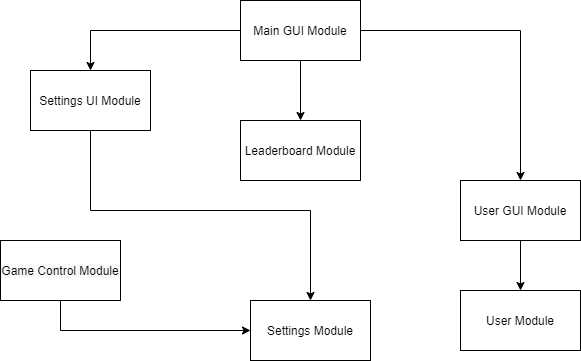
\includegraphics[width=0.7\textwidth]{UsesHierarchy.png}
\caption{Use hierarchy among modules}
\label{FigUH}
\end{figure}

%\section*{References}

\bibliographystyle {plainnat}
\bibliography {MG}

\end{document}
